% ----------------------------------------------------
% Magic Comments for LaTeX-editors (TeXstudio, VSCode with LaTeX Workshop extension...)
% !TeX encoding = utf8
% !TeX spellcheck = de_DE
% !TeX program = pdflatex
% !BIB program = biber
% ----------------------------------------------------

% ----------------------------------------------------
% Load the HfTL-Thesis class
\documentclass[
% Select the main Language of your thesis here. Titlepage, captions and statement of authorship will change accordingly:
%
ngerman % - Deutsch (default)
% USenglish % - American english
% UKenglish % - British english
%
numeric % (default) use numeric citation style sorted by the occurence in text: [5]
% alphabetic % - use alphabetic citation style: [Lau95]
% authoryear % - use authoryear citation style: Laubach 1995
]{Bachelorarbeit}
% ----------------------------------------------------

% ----------------------------------------------------
% Set your custom options here. See https://komascript.de/~mkohm/scrguide.pdf for possibilities.

%\KOMAoption{twoside}{true} % Enable double sided layout
%\KOMAoption{BCOR}{8.25mm} % Binding Correction, adds the specified margin to the inner side of the page (left on single sided layout). This is to compensate lost page margin due to binding.

% ----------------------------------------------------

% ----------------------------------------------------
% Load your own packages here

\usepackage{blindtext} % Only for demonstration purposes. Can be removed!
\usepackage{tikz, pgfplots} % To create diagrams and figures directly with LaTeX
\usepackage{listings} % support for Sourcecodelistings. For more advanced, prettier highlighting use the minted package instead (https://github.com/gpoore/minted) -> Requires Python with Pygments installed.
\usepackage{siunitx} % provides support for SI unit handling
\usepackage[useregional]{datetime2} % support for formatted date
\usepackage{tocstyle} % support indent in table of contents
\usepackage{graphicx}

% Options for table of contents
\usetocstyle{KOMAlike}

% ----------------------------------------------------

% ----------------------------------------------------
% Variables for Titlepage, PDF properties...
% Below are the default values. Comment them out to change them!

\university{Hochschule für Telekommunikation Leipzig (FH)}
\institute{Institut für Telekommunikationsinformatik}
\documentKind{Abschlussarbeit zur Erlangung des akademischen Grades}
\forDegree{Bachelor of Science}
%
\topic{\enquote{Inwiefern bietet die Authentifikation ohne Passwort Vor- und Nachteile gegenüber Webanwendungen hinsichtlich Nutzerfreundlichkeit, Datenschutz und Sicherheit?}}
%
\thesisAuthor{Ertugrul Sener}
\authorDateOfBirth{17.10.1998}
\authorPlaceOfBirth{Berlin}
%
\handInDate{\today} %formatted custom date
%
\firstReviewerName{Prof. Dr. Erik Buchmann}
\firstReviewerInstitution{Hochschule für Telekommunikation Leipzig}
\firstReviewerInstitutionStreet{Gustav-Freytag-Straße 43-45}
\firstReviewerInstitutionPlace{04277 Leipzig}
%
\secondReviewerName{Juri Lobov}
\secondReviewerInstitution{T-Systems International GmBH}
\secondReviewerInstitutionStreet{Holzhauser Straße 1-4}
\secondReviewerInstitutionPlace{13509 Berlin}

% ----------------------------------------------------

% ----------------------------------------------------
% Include own references
\addbibresource{References/online.bib}
\addbibresource{References/3gpp.bib}
%\addbibresource{References/etsi.bib}
\addbibresource{References/itut.bib}
\addbibresource{References/rfc.bib}
% ----------------------------------------------------

% ----------------------------------------------------
% Set a list of directories, where graphics are stored, so you dont have to prepend the subdirectory in \includegraphics. The "Graphics" folder is set by default.

%\graphicspath{{./Graphics/}, {./Images}}
% ----------------------------------------------------

% ----------------------------------------------------
% Load acronym definitions
\newacronym{otp}{OTP}{One time password}
\newacronym{totp}{TOTP}{Time based one time password}
\newacronym{hotp}{HOTP}{HMAC based one time password}
\newacronym{bsi}{BSI}{Bundesamt für Sicherheit in der Informationstechnik}
\newacronym{nist}{NIST}{National Institute of Standards and Technology}
\newacronym{mitm}{MITM}{Man-in-the-middle}
\newacronym{u2f}{U2F}{Universal second factor}
\newacronym{2fa}{2FA}{Zwei-Faktor-Authentifizierung}
\newacronym{isms}{ISMS}{Informationssicherheits-Managementsystem}
\newacronym{ctap}{CTAP}{Client-to-Authenticator protocol}
\newacronym{webauthn}{WebAuthn}{Web Authentication}
\newacronym{rest}{REST}{Respresentational State Transfer}
\newacronym{spa}{SPA}{Single Page Application}
\newacronym{3gpp}{3GPP}{Third Generation Partnership Project}
\newacronym{aaa}{AAA}{Authentication, Authorisation and Accounting}
\newacronym{aac-eld}{AAC-ELD}{Advanced Audio Coding-Enhanced Low Delay}
\newacronym{acr}{ACR}{Absolute Category Rating}
\newacronym{af}{AF}{Application Function}
\newacronym{agcf}{AGCF}{Access Gateway Control Function}
\newacronym{agch}{AGCH}{Access Grant Channel}
\newacronym{ajax}{AJAX}{Asynchronous JavaScript and XML}
\newacronym{amr}{AMR}{Adaptive Multi Rate}
\newacronym{amr-wb}{AMR-WB}{Adaptive Multirate-Wideband}
\newacronym{ape}{APE}{AJAX Push Engine}
\newacronym{api}{API}{Application Programming Interface}
\newacronym{apn}{APN}{Access Point Name}
\newacronym{appserv}{AS}{Application Server}
\newacronym{armgw}{A/R-MGW}{Access/Residential-Media Gateway}
\newacronym{arvgw}{A/R-VGW}{Access/Residential-Voice over IP-Gateway}
\newacronym{as}{AS}{Access Stratum}
\newacronym{auc}{AuC}{Authentication Centre}
\newacronym{avp}{AVP}{Attribute-Value-Pairs}
\newacronym{bcch}{BCCH}{Broadcast Control Channel}
\newacronym{bgcf}{BGCF}{B bsreakout Gateway Control Function}
\newacronym{bsc}{BSC}{Base Station Controller}
\newacronym{bts}{BTS}{Base Transceiver Station}
\newacronym{ca}{CA}{Certificate Authority}
\newacronym{ca_mac}{CA}{Collision Avoidance}
\newacronym{camel}{CAMEL}{Customised Application for Mobile network Enhanced Logic}
\newacronym{cc}{CC}{Call Control, Country Code}
\newacronym{celp}{CELP}{Code-Excited Linear-Prediction}
\newacronym{celt}{CELT}{Constrained Energy Lapped Transform}
\newacronym{cli}{CLI}{Command Line Interface}
\newacronym{cm}{CM}{Connection Management}
\newacronym{cng}{CNG}{Comfort Noise Generation}
\newacronym{cod}{CoD}{Content on Demand}
\newacronym{cp}{CP}{Control Plane}
\newacronym{cpe}{CPE}{Customer-Premises Equipment}
\newacronym{cs}{CS}{Circuit Switched}
\newacronym{cs-acelp}{CS-ACELP}{Conjugate-Structure Algebraic-Code Excited Linear-Prediction}
\newacronym{cscf}{CSCF}{Call/Session Control Function}
\newacronym{csfb}{CSFB}{Circuit Switched Fallback}
\newacronym{csma}{CSMA}{Carrier Sense Medium Access}
\newacronym{css}{CSS}{Cascading Style Sheets}
\newacronym{db}{DB}{Database}
\newacronym{dom}{DOM}{Document Object Model}
\newacronym{dscp}{DSCP}{Differentiated Services Code Points}
\newacronym{dtls}{DTLS}{Datagram Transport Layer Security}
\newacronym{dtx}{DTX}{Discontinuous Transmission}
\newacronym{dv}{DV}{Delay Variation}
\newacronym{e-rab}{E-RAB}{E-UTRAN Radio Access Bearer}
\newacronym{e-utran}{E-UTRAN}{Evolved UMTS Radio Access Network}
\newacronym{e2e}{E2E}{End-to-End}
\newacronym{edge}{EDGE}{Enhanced Data rates for GSM Evolution}
\newacronym{edss1}{EDSS1}{European Digital Subscriber System No. 1}
\newacronym{eir}{EIR}{Equipment Identity Centre, Equipment Identity Register}
\newacronym{epc}{EPC}{Evolved Packet Core}
\newacronym{epg}{EPG}{Electronic Program Guide}
\newacronym{eps}{EPS}{Evolved Packet System}
\newacronym{etsi}{ETSI}{European Telecommunication Standards Institute}
\newacronym{etsi-tispan}{ETSI-TISPAN}{ETSI-Telecommunications and Internet converged Services and Protocols for AdvancedNetworking}
\newacronym{facch}{FACCH}{Fast Associated Control CHannel}
\newacronym{fb}{FB}{Fullband}
\newacronym{fcch}{FCCH}{Frequency Correction CHannel}
\newacronym{fec}{FEC}{Forward Error Correction}
\newacronym{fmc}{FMC}{Fixed Mobile Convergence}
\newacronym{fokus}{FOKUS}{Fraunhofer-Institut für Offene Kommunikationssysteme}
\newacronym{fr}{FR}{Full Rate}
\newacronym{geran}{GERAN}{GSM EDGE Radio Access Network}
\newacronym{ggsn}{GGSN}{Gateway GPRS Support Node}
\newacronym{gmm}{GMM}{GPRS Mobility Management}
\newacronym{gmsc}{GMSC}{Gateway MSC}
\newacronym{gprs}{GPRS}{General Packet Radio Service}
\newacronym{gsm}{GSM}{Global System for Mobile communications}
\newacronym{gsma}{GSMA}{GSM Association}
\newacronym{gtp}{GTP}{GPRS Tunneling Protocol}
\newacronym{gui}{GUI}{Graphical User Interface}
\newacronym{gw}{GW}{Gateway}
\newacronym{hd}{HD}{High Definition}
\newacronym{hlr}{HLR}{Home Location Register}
\newacronym{hr}{HR}{Half Rate}
\newacronym{hscsd}{HSCSD}{High-Speed Circuit-Switched Data}
\newacronym{hss}{HSS}{Home Subscriber Server}
\newacronym{html5}{HTML5}{Hypertext Markup Language Version 5}
\newacronym{http}{HTTP}{Hypertext Transfer Protocol}
\newacronym{https}{HTTPS}{Hypertext Transfer Protocol Secure}
\newacronym{iad}{IAD}{Integrated Access Device}
\newacronym{iana}{IANA}{Internet Assigned Numbers Authority}
\newacronym{ibcf}{IBCF}{Interconnection Border Control Function}
\newacronym{ibgf}{IBGF}{Interconnection Border Gateway Function}
\newacronym{ice}{ICE}{Interactive Connectivity Establishment}
\newacronym{i-cscf}{I-CSCF}{Interrogating-CSCF}
\newacronym{iesg}{IESG}{Internet Engineering Steering Group}
\newacronym{ietf}{IETF}{Internet Engineering Task Force}
\newacronym{imei}{IMEI}{International Mobile Equipment Identity}
\newacronym{ims}{IMS}{IP Multimedia Subsystem}
\newacronym{imscm}{IMSCM}{IMS-Client-Manager}
\newacronym{imsi}{IMSI}{International Mobile Subscriber Identity}
\newacronym{imssf}{IM-SSF}{IP Multimedia Service Switching Function}
\newacronym{imt}{IMT}{International Mobile Telecomunication}
\newacronym{inap}{INAP}{Intelligent Network Application Part}
\newacronym{ip}{IP}{Internet Protocol}
\newacronym{ip-can}{IP-CAN}{Internet Protocol- Connectivity Access Network}
\newacronym{ipdv}{IPDV}{IP Delay Variation}
\newacronym{iper}{IPER}{IP Packet Error Ratio}
\newacronym{iplr}{IPLR}{IP Packet Loss Ratio}
\newacronym{iptd}{IPTD}{IP Transfer Delay}
\newacronym{iptv}{IPTV}{Internet Protocol Television}
\newacronym{isc}{ISC}{IMS Service Control}
\newacronym{isdn}{ISDN}{Integrated Services Digital Network}
\newacronym{iso/osi}{ISO/OSI}{Open System Interconnection/International Organization for Standardization}
\newacronym{isup}{ISUP}{ISDN User Part}
\newacronym{itu}{ITU}{International Telecommunication Union}
\newacronym{itu-t}{ITU-T}{International Telecommunications Union-Telecommunication Standardization Sector}
\newacronym{json}{JSON}{JavaScript Object Notation}
\newacronym{la}{LA}{Location Area}
\newacronym{label}{API}{Application Programming Interface}
\newacronym{lcp}{LCP}{Link Control Protocol}
\newacronym{llc}{LLC}{Logical Link Control}
\newacronym{lp}{LP}{Linear Prediction}
\newacronym{lte}{LTE}{Long Term Evolution}
\newacronym{m2m}{M2M}{Machine to Machine Communication}
\newacronym{mac}{MAC}{Medium Access Control}
\newacronym{mac_encryption}{MAC}{Message Authentication Code (encryption context)}
\newacronym{map}{MAP}{Mobile Application Part}
\newacronym{mcf}{MCF}{Media Control Function}
\newacronym{mdct}{MDCT}{Modified Discrete Cosine Transform}
\newacronym{mdf}{MDF}{Media Delivery Function}
\newacronym{mfv}{MFV}{Mehrfach Frequenz Wahlverfahren/Tonwahl}
\newacronym{mgc}{MGC}{Media Gateway Controler}
\newacronym{mgcf}{MGCF}{Media Gateway Control Function}
\newacronym{mgw}{MGW}{Media Gateway Function}
\newacronym{mime}{MIME}{Multipurpose Internet Mail Extensions}
\newacronym{mm}{MM}{Mobility Management}
\newacronym{mme}{MME}{Mobile Management Entity}
\newacronym{mos}{MOS}{Mean Opinion Score}
\newacronym{mrf}{MRF}{Multimedia Resource Function}
\newacronym{mrfc}{MRFC}{Multimedia Resource Function Controller}
\newacronym{mrfp}{MRFP}{Multimedia Resource Function Processor}
\newacronym{ms}{MS}{Mobile Station}
\newacronym{msc}{MSC}{Mobile Switching Centre}
\newacronym{msisdn}{MSISDN}{Mobile Subscriber ISDN Number}
\newacronym{n-pvr}{N-PVR}{Network-Personal Video Recorder}
\newacronym{napt}{NAPT}{Network Address and Port Translation}
\newacronym{nas}{NAS}{Non-Access Stratum}
\newacronym{nas_server}{NAS}{Network Access Server}
\newacronym{nass}{NASS}{Network Attachment Subsystem}
\newacronym{nat}{NAT}{Network Address Translation}
\newacronym{nb}{NB}{Narrowband}
\newacronym{nfv}{NFV}{Network Function Virtualization}
\newacronym{ngn}{NGN}{Next Generation Network}
\newacronym{nni}{NNI}{Network-Network Interface}
\newacronym{nodeb}{NodeB}{Funkbasisstation im UTRAN}
\newacronym{nsapi}{NSAPI}{Network Service Access Point Identifier}
\newacronym{ntba}{NTBA}{Network Termination for ISDN Basic rate Access / Netzterminator Basisanschluss}
\newacronym{osa}{OSA}{Open Service Access}
\newacronym{osascs}{OSA-SCS}{Open Service Access - Service Capability Server}
\newacronym{osgi}{OSGi}{Open Services Gateway initiative}
\newacronym{osi}{OSI}{Open System Interconnection}
\newacronym{ott}{OTT}{Over The Top Anwendungen}
\newacronym{p-cscf}{P-CSCF}{Proxy Call Session Control Function}
\newacronym{pcc}{PCC}{Policy and Charging Control}
\newacronym{pcef}{PCEF}{Policy Control Enforcement Function}
\newacronym{pch}{PCH}{Paging Channel}
\newacronym{pcrf}{PCRF}{Policy and Charging Rules Function}
\newacronym{pcu}{PCU}{Packet Control Unit}
\newacronym{pdn}{PDN}{Public Data Network, Packet Data Network}
\newacronym{pdn-gw}{PDN-GW}{Packet Data Network Gateway}
\newacronym{pelr}{PELR}{Packet Error Loss Rate}
\newacronym{pes}{PES}{PSTN/ISDN Emulation Subsystem}
\newacronym{pesq}{PESQ}{Perceptual Evaluation of Speech Quality}
\newacronym{pgw}{PGW}{Packet Data Network Gateway}
\newacronym{php}{PHP}{PHP: Hypertext Preprocessor}
\newacronym{plmn}{PLMN}{Public Land Mobile Network}
\newacronym{plr}{PLR}{Packet Loss Rate}
\newacronym{pnai}{PNAI}{Personal Network Administration Interface}
\newacronym{polqa}{POLQA}{Perceptual Objective Listening Quality Assessment}
\newacronym{pots}{POTS}{Plain Old Telephone System}
\newacronym{ppv}{PPV}{Pay-Per-View}
\newacronym{ps}{PS}{Packet Switched, Location Probability}
\newacronym{pss}{PSS}{PSTN/ISDN Simulation Subsystem}
\newacronym{pstn}{PSTN}{Public Switched Telephone Network}
\newacronym{qci}{QCI}{QoS Class Identifier}
\newacronym{qoe}{QoE}{Quality of Experience}
\newacronym{qos}{QoS}{Quality of Service}
\newacronym{ra}{RA}{Routing Area, Random mode request information field}
\newacronym{rab}{RAB}{Radio Access Bearer, Access Burst}
\newacronym{rat}{RAT}{Radio Access Technology}
\newacronym{rach}{RACH}{Random Access Channel}
\newacronym{racs}{RACS}{Resource Admission Control Subsystem}
\newacronym{radius}{RADIUS}{Remote Authentication Dial In User Service}
\newacronym{rcs}{RCS}{Rich Communication Suite}
\newacronym{rlc}{RLC}{Radio Link Control}
\newacronym{rnc}{RNC}{Radio Network Controller}
\newacronym{rpe-ltp}{RPE-LTP}{Regular Pulse Excitation - Long Term Prediction}
\newacronym{rr}{RR}{Radio Resources}
\newacronym{rrc}{RRC}{Radio Resource Control}
\newacronym{rtc}{RTC}{Real Time Communication}
\newacronym{rtcp}{RTCP}{RTP Control Protocol}
\newacronym{rtp}{RTP}{Realtime Transport Protocol}
\newacronym{rtsp}{RTSP}{Real-Time Streaming Protocol}
\newacronym{rtt}{RTT}{Round Trip Time}
\newacronym{sacch}{SACCH}{Slow Associated Control Channel}
\newacronym{sai}{SAI}{Service Attachment Information}
\newacronym{sapi}{SAPI}{Service Access Point Identifier}
\newacronym{scf}{SCF}{Service Control Function}
\newacronym{sch}{SCH}{Synchronisation Channel}
\newacronym{s-cscf}{S-CSCF}{Serving-CSCF}
\newacronym{sctp}{SCTP}{Stream Control Transmission Protocol}
\newacronym{sd}{SD}{Standard Definition}
\newacronym{sdcch}{SDCCH}{Stand-Alone Dedicated Control Channel}
\newacronym{sdf}{SDF}{Service Discovery Function}
\newacronym{sdma}{SDMA}{Space Division Multiple Access}
\newacronym{sdp}{SDP}{Session Description Protocol}
\newacronym{servgw}{ServGW}{Serving Gateway}
\newacronym{sgsn}{SGSN}{Serving GPRS Support Node}
\newacronym{sgw}{S-GW}{Signaling Gateway}
\newacronym{sigtran}{SIGTRAN}{ZGSNr.7 Signaling Transport Protocol Suite}
\newacronym{silk}{SILK}{SILK Speech codec}
\newacronym{sip}{SIP}{Session Initiation Protocol}
\newacronym{sipas}{SIP AS}{SIP Application Server}
\newacronym{slf}{SLF}{Subscriber Location Function}
\newacronym{sms}{SMS}{Short Message Service}
\newacronym{srtp}{SRTP}{Secure Real-Time Transport Protocol}
\newacronym{ss}{SS}{Supplementary Service}
\newacronym{sscon}{SSCON}{Session Controller}
\newacronym{ssf}{SSF}{Service Selection Function}
\newacronym{ssi}{SSI}{Service Selection Information}
\newacronym{ssrc}{SSRC}{Synchronization Source}
\newacronym{stun}{STUN}{Session Traversal Utilities for NAT}
\newacronym{swb}{SWB}{Super-Wideband}
\newacronym{tch}{TCH}{Traffic Channel}
\newacronym{tcp}{TCP}{Transmission Control Protocol}
\newacronym{td}{TD}{Transfer Delay}
\newacronym{tdd}{TDD}{Time Division Duplex}
\newacronym{tispan}{TISPAN}{Telecommunications and Internet converged Services and Protocols for Advanced Networking}
\newacronym{tmsi}{TMSI}{Temporary Mobile Subscriber Identity}
\newacronym{tn}{TN}{Termination Node, Timeslot Number}
\newacronym{toc}{TOC}{Table-Of-Contents}
\newacronym{turn}{TURN}{Traversal Using Relays around NAT}
\newacronym{tv}{TV}{Television}
\newacronym{ua}{UA}{User Agent}
\newacronym{udp}{UDP}{User Datagram Protocol}
\newacronym{ue}{UE}{User Equipment}
\newacronym{umts}{UMTS}{Universal Mobile Telecommunications System}
\newacronym{uni}{UNI}{User-Network Interface}
\newacronym{up}{UP}{User Plane}
\newacronym{upsf}{UPSF}{User Profile Server Function}
\newacronym{uri}{URI}{Uniform Resource Identifier}
\newacronym{url}{URL}{Uniform Resource Locator}
\newacronym{utran}{UTRAN}{Universal Terrestrial Radio Access Network}
\newacronym{vad}{VAD}{Voice Activity Dedection}
\newacronym{vbr}{VBR}{Variable Bit  Rate}
\newacronym{vgw}{VGW}{Voice over IP-Gateway}
\newacronym{vlc}{VLC}{VideoLan Client}
\newacronym{vod}{VoD}{Video on Demand}
\newacronym{voip}{VoIP}{Voice Over IP}
\newacronym{volga}{VoLGA}{Voice over LTE via Generic Access}
\newacronym{volte}{VoLTE}{Voice over LTE}
\newacronym{w3c}{W3C}{World Wide Web Consortium}
\newacronym{waf}{WAF}{WebRTC Authentication Function}
\newacronym{wb}{WB}{Wideband}
\newacronym{webrtc}{WebRTC}{Web Real-Time Communication}
\newacronym{wlan}{WLAN}{Wireless Local Area Network}
\newacronym{wqsf}{WQSF}{WebRTC QoS Signalling Function}
\newacronym{wwsf}{WWSF}{WebRTC Web Server Function}
\newacronym{xdsl}{xDSL}{any Digital Subscriber Line}
\newacronym{xml}{XML}{Extended MarkupLanguage}
\newacronym{zgs nr.7}{ZGS Nr.7}{Zentrales Zeichengabesystem Nr.7}

\makenoidxglossaries % index acronyms
% ----------------------------------------------------

% ----------------------------------------------------
% The document body. Start your work here.
\begin{document}
% \frontmatter % page numbers as small roman letters
\maketitle % print the titlepage
\cleardoublepage % start a new page

\chapter{Vorwort}
Hier is

\blindtext
 % include the file Content/vorwort.tex
\cleardoublepage

\makedeclarationofauthorship % print the declaration of authorship

\tableofcontents %print the table of contents
\cleardoublepage

\printnoidxglossary[type=\acronymtype] % print the list of abbreviations
\cleardoublepage

\listoffigures % print the list of figures
\cleardoublepage

\listoftables % print the list of tables
\cleardoublepage

\lstlistoflistings % print the list of source codes
\cleardoublepage	

% Include the other chapters
% !TeX root = ../Bachelorarbeit.tex
\chapter{Einleitung}

\section{Motivation}
Die Motivation für die Erarbeitung der Forschungsfrage ergab sich am 19. Juli 2020, als eine Rundmail des Data Breach Monitoring-Tools von Firefox die Bildschirme erreichte, welches einen neuen Incident bei Wattpad meldete [A16]. Nun stellt sich die berechtigte Frage, inwiefern diese in Relation kleine Webseite verwertbare Daten für einen Angreifer oder ein bösartiges Tool liefern kann. Dazu genügt es sich die Daten genauer anzusehen. Kompromittiert wurden neben den klassichen Daten wie Passwörtern, IP-Adressen, E-Mail-Adressen und Geburtsdaten auch sehr persönliche Informationen wie geografische Standorte, ein Kurzprofil des Nutzers und die Social-Media-Profile der Nutzer [A16]. Entnehmen kann man dies mehreren Artikeln, bei der die Angabe nach der Größe der Datenmengen zwischen 250 und 280 Millionen Einträgen variiert [A17, A18]. Eine genaue Zahl liefert der Artikel der riskbasedsecurity mit 268.830.266 (nach der Entfernung von Duplikaten) kompromittierten E-Mail Addressen, die sich laut des Artikels in einer einzigen Datenbank befanden \cite{A6}. Diese Zahl ist dennoch nur als Richtwert zu verstehen, da das Ausmaß des Datenlecks bei Wattpad nicht in Gänze bekannt ist.

\section{Problemdefinition}
Mit dem Passwort gelangt der Angreifer an die Identität des Nutzers.  Identitätsdiebstahl sei laut BSI ein alltägliches Phänomen, dass jeden Monat eine große Anzahl an digitalen Identitäten von Privatanwendern betrifft [A19]. Es ist allgemein bekannt, dass Daten die im Internet landen kaum oder nur mit erheblichem Mehraufwand aus diesem vollständig entfernbar sind. Die Identität kann nun für missbräuchliche Zwecke entfremdet und missbraucht werden.
\newpage

Auch wenn es bei der Bekanntmachung und Berichterstattung zu solchen Datenlecks manchmal so scheint, ist auch dieses nicht das einzige Beispiel für kompromittierte Unternehmen der letzten Zeit [A20]. Gegen Angriffe auf die Technik (beispielsweise Code-Injektionen, 0-Day-Exploits oder Bruteforce-Angriffe) scheint die informationsaffine Menscheit der Neuzeit gut organisiert zu sein, doch dann scheitert es an der Wahl des richtigen Passwortes. Passwörter wichtiger Personen innerhalb eines Unternehmens können nun ohne große Mühen über die Google Suchergebnisse gefunden werden. So liefert die Anfrage 'allintext:password filetype:log after:2019' auf Google alle Logdateien nach 2019, die den Schlüssel ``password'' beeinhalten. Alternativ kann man  über Anfragen folgender Art: 'wattpad data breach download' gezielt nach einem Downloadlink für spezielle Data Breaches suchen. Solche Listen werden häufig in unbekannteren Foren geteilt.Meistens erscheinen Username und Passwort im Format 'Username:Passwort', der erste Doppelpunkt trennt demnach die beiden Zeichenketten. Der Zeilenumbruch trennt die unterschiedlichen Accounts.

Die Passwörter dieser Personen sind im Regelfalle nicht im Klartext aus dem Breach entnommen worden, sondern wurden mittels Hashkillers gebruteforced. Hashkiller sind Passwortcrackingtools die für häufig genutze Hashingalgorithmen wie md5 oder sha256 Milliarden von Ergebnissen vorberechnen um bei entsprechender Suche über den Hash an den Klartext zu gelangen. Dies funktioniert besonders häufig bei sehr einfachen Passwörtern, die in diesen Tabellen sind und am Ende als Klartext dann in solchen Foren verteilt werden.

Ein Grund gegen die Nutzung von externen Geräten für die zwei Faktor Authentifizierung ist die Folge bei Verlust des Gerätes, mit dem die Webseite gekoppelt ist. Dies bedeutet den Verlust des gekoppelten Accounts. Ohne entsprechende Backup-Codes kann womöglich kein Zugang mehr gewährt werden, da das Zurücksetzen des Passwortes meist auch die Authentifizierung durch den zweiten Faktor benötigt so wie zum Beispiel bei Windows Outlook. Ein User besteht auf seine Bequemlichkeit und will so schnell wie möglich und ohne Zwischenschritte Zugang zu seinen Diensten erhalten. Ein zweiter Faktor bedeutet das nach Eingabe des Passwortes das Smartphone gesucht, womöglich noch entsperrt, die zugehörige App geöffnet und die Sicherungen (PIN, Fingerabdruck, Gesichtsmerkmale) an den Server übertragen und verarbeitet werden müssen.
\newpage

Das Speichern von allen Passwörtern, durch einen Passwort-Manager, an einem gesammelten Ort muss ``mit einem gut gewählten Master-Passwort geschützt sein`` [A21]. Der Verlust des Masterpasswortes würde den Verlust aller Daten (und den an ihnen hängenden digitalen Identitäten) des Nutzers bedeuten. Die Frage, die sich stellt ist es, ob man mit einer Kombination aus den vorhandenen vielfältigen Authentifizierungsmöglichkeiten eine bequeme aber gleichzeitig sichere Authentifizierungsvariante schaffen kann, bei denen es dem Anwender möglich sein soll, sich gegenüber einer Webseite zu authentifizieren.

\section{Stand der Forschung}
\subsection{Bequemlichkeitsproblem}
Bei einem Angriff ist es nicht zwingend notwendig, dass die Authentifizierungsquelle, also jene Quelle bei der die Daten persistiert sind und die die Authentifizierung bei Eingabe durchführt, diese Daten durch fehlerhafte Programmierung herausgibt. Durch sogenannte Metadaten, das sind Informationen und Merkmale zu Daten, ist es Angreifern häufig möglich das Passwort zu erraten bzw. zurückzusetzen. Wenn also der Benutzername lautet 'MichaelJacksonFanForever' ist die Antwort auf die Sicherheitsfrage zum Lieblingskünstler nicht weit entfernt.

Gleichzeitig neigen Menschen aufgrund von Bequemlichkeit zu leicht merkbaren Passwörtern, die sie mehrfach für verschiedene Dienste verwenden. Das die Passwortproblematik allgegenwärtig ist, stützt eine durchgeführte repräsentative Studie der Bitkom Research \cite{A1} im Auftrag des Digitalverbands Bitkom. So nutze etwa jeder dritte Onlinenutzer (36\%) dasselbe Passwort für mehrere Dienste. Auch wenn gleichzeitig 63\% der Befragten angaben, bei der Erstellung von Passwörtern auf ``einen Mix aus Buchstaben, Zahlen und Sonderzeichen'' \cite{A1} zu achten. Eine ähnliche Studie hat die Bitkom zum Thema 'Nachlässigkeit bei Passwörtern' am 08.11.2016 \cite{A2} gemacht, bei der die prozentuale Verteilung an unsicheren Passwortnutzern die befragt wurden nur einen Prozent höher liegt. Das heißt konkret, dass sich innerhalb von 4 Jahren keine messbare Besserung ergeben hat. Das Bewusstsein über die Internetpräsenz und der Schutz dessen scheinen immernoch keine große Aufmerksamkeit vom modernen Nutzer zu erhalten. Das Problem mit unsicheren Passwörtern ist allerdings so alt wie das Internet.

\subsection{Unsichere Passwörter}
Der Begriff des Passwortes entstammt dem militärischen Bereich des 16. Jahrhunderts, wobei tatsächlich das einzelne Wort adressiert war, welches einem Zutritt zu Gebäuden verschaffte. Damit verwandt ist das Kennwort, welches nicht das Passieren sondern die Kennung des gemeinsamen Geheimnisses betont. Dies bedeutet, dass der Passierer mit einem Kennwort auch automatisch ein Geheimnisträger ist. Als Computer immer leistungsfähiger wurden, wurde der Begriff der Passphrase etabliert, um die Notwendigkeit längerer Passwörter hervorzuheben. Weitere Schlüsselwörter für das heutzutage bekannte Passwort sind: Schlüsselwort, Kodewort (Codewort) oder die Parole, diese werden im Folgenden als Synonym für die heutige Passphrase verwendet.

User verwenden häufig das selbe leicht zu erratende Passwort für mehrere Accounts auf unterschiedlichen Diensten \cite{A3}. Die Länge entscheidet mitunter über die Sicherheit von Passwörtern. Allgemein gillt: je länger desto besser \cite{A4}. Dies muss allerdings nicht grundsätzlich der Fall sein, denn laut BSI könne ein starkes Passwort kürzer und komplex oder lang und weniger komplex sein \cite{A4}. Anhand sogenannter Passwort-Policies, das sind Regeln für Passwörter, machen die Webseiten das Wählen von Passwörtern komplizierter. Dabei umfasst die Password Policy gängige Festlegungen wie die Mindestlänge, die Komplexität und die Lebensdauer \cite{A3}. Außerdem gibt es die Möglichkeit des Verbot von sich wiederholenden Zeichenketten wie ''testtest``, längeren Zahlenreihenwiederholungen wie ''123123`` oder dem Verbot der Nutzung des Usernamen im Passwort. Das gewählte Passwort soll für einen selbst leicht merkbar, für einen Computer oder menschlichen Angreifer schwer zu erraten sein.

Ferner sind der Kreativität von Passwörtern laut \ac{bsi} keine Grenzen gesetzt \cite{A4}. Zum Beispiel könne man einen leicht zu merkenden Satz nehmen, diesen mit Bindestrichen verbinden und von jedem Wort den ersten Buchstaben entfernen. Die Frage die sich dabei stellt ist es, ob dieser Satz dann die Tippgeschwindigkeit des Nutzers beeinträchtigt, weil relativ viele Denkprozesse während des Tippens stattfinden müssen. Zunächst ein Mal müsste sich hierbei der Satz in voller länge gemerkt werden, dies ist noch Recht unkompliziert für den allgemeinen Internetnutzer. Danach muss der Satz während des Tippens bereits mit Bindestrichen verbunden werden, auch dies ist noch kein großen Problem. Zum Problem wird es, sich die ersten Buchstaben beim Tippen automatisch wegzudenken, sodass einem kein Fehler unterläuft. Wenn einem doch ein Fehler unterläuft, ist es anders als bei gängigen Passwörtern, sehr schwer zur Fehlerquelle zu springen und den Fehler zu lokalisieren.
\newpage

Alternativ bleibt einem nur das Neutippen des Passwortes, welches eine große Zeitverzögerung für den Nutzer bedeutet und auf lange Sicht den Nutzer dazu bringen wird, ein einfacheres und leicht tippbares Passwort zu wählen.

Webseiten nutzen typischerweise standardisierte und gleiche Regeln für jeden Nutzer, doch ignorieren den Fakt, dass jeder Nutzer andere Präferenzen besitzt. Dies macht es schwierig, die Ziele dieser 'strong password goals' zu erreichen. Um die Effektivität für diese Methoden zu steigern, wird eine \ac{dppp} empfohlen. Diese kann auf den Charakterzügen des Nutzers basierend personalisierte Password Policies vorschlagen. [A22] Diese passen sich dem Nutzer an und lösen das Problem der Usability im Bereich der Password Policies.

Ferner können Passwort Policys wertvolle Informationen für einen potenziellen Angreifer bieten. Denn was Angreifer durch sehr strikte Passwort Policys unteranderem erkennen können, ist die Mindest- und Maximalzeichenlänge. Dabei wird der Angreifer zum Beispiel aus der Regel 'Das Passwort muss mindestens 8 und maximal 16 Zeichen lang sein.' alle Kombinationen für weniger als 8 Zeichen und mehr als 16 Zeichen bei der Erratung eliminieren können. Weitere Regeln wie 'Das Passwort muss mindestens ein Sonderzeichen beinhalten' können zusätzliche Informationen bieten. Daher sind Passwort-Policys zwar ein sehr wichtiges Werkzeug, um Nutzer zu sicheren Passwörtern zu zwingen. Durch die beeinträchtigte Bequemlichkeit in der freien Passwortwahl des Nutzers können dennoch einfach zu erratende Passwörter gewählt werden, die den Kriterien entsprechen. Verhindern lässt sich dies nicht ganz. Die Informationen die Nutzer beim Anmelden bekommen, nutzen Angreifer dann zum Knacken jener Passwörter. Aus Sicht des Angreifers lautet die Faustregel: Je mehr Metadaten, desto besser.
\newpage

\subsection{Übertragungsproblem}
Das Problem mit der Unsicherheit von Passphrasen oder Passwörtern beginnt jedes Mal aufs Neue, sobald man ein Passwort eintippt. So ist die Bedrohung nicht mit der Wahl eines mathematisch sicheren Passwortes gebannt. Das Verfahren der Passwortauthentifikation bedient sich prinzipiell einer Zeichenkette, die man in ein Feld eintippt und ist per se dann unsicher sobald einer der Geheimnisträger (Menschen mit Kenntniss über die Parole) kompromittiert bzw. infiziert ist. So gibt es verschiedenste Angriffsvektoren um das Passwort eines Users für einen speziellen Dienst herrauszufinden. Von personalisierten (oder auch allgemeinen) Phishing Mails, zu Shoulder Surfing bis hin zu Trojanern und Keyloggern auf dem System Desjenigen, der es zum Zeitpunkt des Angriffs in die Tastatur tippt. Die genannten Angriffsmöglichkeiten können nicht alle remote ausgeführt werden. So benötigt es für das Shoulder Surfing und USB-Sticks die Trojaner beinhalten physischen Zugang zum System oder die körperliche Nähe zu der Person, die das System regulär verwaltet. Ein weiteres großes Problem ist die Übertragung von Passwörtern über die klassiche User-Browser-Schnittstelle. Dabei wird das Passwort im Browser des Clients gehasht und dann an den Server übertragen. Die sichere Kommunikation anhand des \ac{https} findet erst bei der Übertragung zum Server statt, die Eingabe des Passwortes an den Browser ist ungeschützt. Diese Übertragung von Buchstaben kann mitgelesen werden.

Das Hashen der Zeichenkette kann in einem ungesicherten Netz sicherlich hilfreich sein, da nun ein Angreifer innerhalb des Netzes das Passwort im Klartext nicht lesen kann. Alles was jener Angreifer sieht, ist der Hash, der auf Clientseite erzeugt wurde und im Request steht. Die Nutzung von \ac{https} macht es zudem noch schwieriger für Angreifer Kommunikationen zwischen User und Server mitzulesen und infolge dessen zu manipulieren. Bei sicheren Verbindungen ist mitunter das Hashing der Nutzerdaten demnach theoretisch nicht mehr nötig. In der Praxis kommt es häufiger vor, dass Zertifikate auf dem Browser des Users installiert werden, die vom Angreifer selbst ausgestellt wurden. Der Durchschnittsnutzer achtet nicht darauf, wer das Zertifikat ausgestellt hat und bekommt womöglich nichts von einem Angriff mit. Solche Zertifikate können in Massen durch eine kompromittierte Root-CA (Certificate Authority) erstellt werden. Root-CA's stellen im wesentlichen Zertifikate aus und prüfen die Identität (und Angaben) des Anforderers eines Zertifikats. Dabei kann es Monate oder sogar Jahre dauern bis gefälschte Zertifikate von einem Nutzer zufällig erkannt, gemeldet und im Anschluss zurückgezogen werden. Ein solcher \ac{mitm} - Angriff auf SSL-Verbindungen ist sehr typisch und wird im folgenden an einer verschlüsselten Verbindung zu einem Webshop sequenziell erläutert.

\begin{figure}[ht]
	\centering
	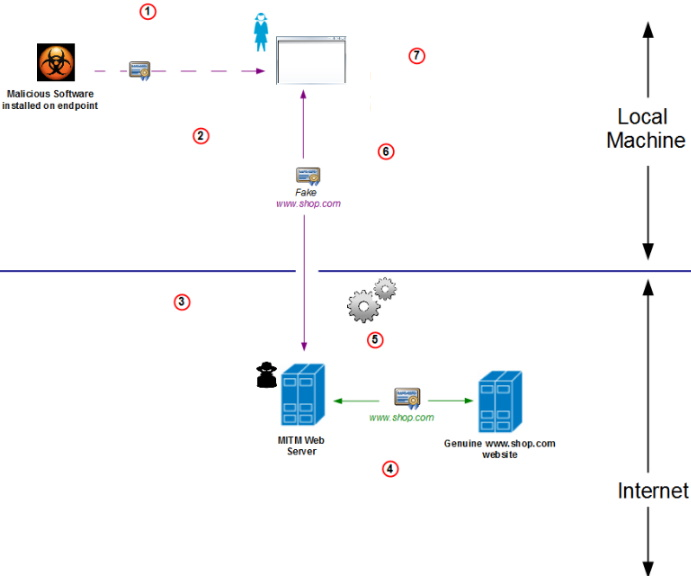
\includegraphics [width=15cm]{mitm_no_CISE.jpg}
	\caption[Man in the middle - Angriff auf SSL verschlüsselte Verbindungen]{MITM - Angriff auf SSL verschlüsselte Verbindungen}
	\label{fig:mitm_no_cise}
\end{figure}

\begin{enumerate} 
\item Im ersten Schritt muss der Angreifer ein eigenes Fake-Zertifikat (im folgenden \ac{mitm}-Zertifikat genannt) im Zertifikatsspeicher des Nutzers installieren. Dies kann eine Malware oder sonstige Fremdsoftware machen. Hat man als Angreifer phsysischen Zugriff zum Rechner, kann man dies innerhalb von wenigen Sekunden selbst machen, ohne dass der Nutzer davon etwas mitbekommt. Der \ac{mitm} - Angriff basiert auf diesem \ac{mitm}-Zertifikat, das von einem potenziellen Angreifer im Namen einer Webseite fälschlicherweise ausgestellt wurde. Ohne diesen Schritt funktioniert der Angriff nicht.
\item Der User möchte eine Verbindung zum Webshop (im Schaubild www.shop.com) aufbauen. Hierzu ruft er die Seite mit dem Präfix https:// auf im Glauben, eine sichere Verbindung aufbauen zu können, die von keinem Dritten mitgelesen werden kann. Der \ac{mitm} fängt die Anfrage ab und leitet ihn zu seinem eigenen Webserver weiter.
\newpage
\item Der Webserver erkennt einen \ac{https} - Request und entschlüsselt mit dem eigenen privaten Schlüssel. Dies kann er durch die Installation der Fake-Root-CA in Schritt 1. Dort wurde die Nachricht mit dem öffentlichen Schlüssel des Angreifers verschlüsselt und abgesendet.
\item Simultan baut der MITM-Webserver eine Verbindung zum echten Webshop auf und leitet die Daten des Nutzers jeweils in beide Richtungen weiter. Dabei simuliert er eine gewöhnliche Nutzeranfrage, die der Webshop nicht als fälschlich erkennen kann. Der User hingegen merkt nichts von dem Angreifer, da er die gewohnte (dies ist Standard) Webseite angezeigt bekommt und keine Annomalien erkennt.
\item Der gesamte Traffic, der eigentlich verschlüsselt sein sollte, kann vom \ac{mitm} mitgelesen, weitergeleitet oder manipuliert werden. Die Verbindung zwischen User und dem Webshop ist nicht sicher trotz \ac{https} Anzeige im Browser.
\item Die Response vom Webshop wird mit dem erstellten MITM-Zertifikat für www.shop.com verschlüsselt und an den User übertragen.
\item Der Browser markiert die Verbindung als sicher und unbedenklich.
\end{enumerate}

Der Nachteil für den Angreifer in diesem Szenario ist die zeitlich limitierte Möglichkeit eines Angriffs. Es muss also auf den initialen Request des Users gewartet werden, um dessen Daten abzufangen und den Prozess des Angriffs in Gang zu setzen. Wiederholungsangriffe (auch: Replay-Attacks) werden in diesem Szenario nicht verhindert. Der Angreifer muss womöglich demnach nicht einmal das Passwort im Klartext besitzen. Es genügt, den Hash und den Benutzernamen im Request abzufangen um diese dann in einem seperaten Aufruf vom eigenen Rechner an die selbe \ac{url} zu senden. Es handelt sich bei dieser Art des Angriffs um das Imitieren von Benutzereingaben durch einen Angreifer, bei der der Angreifer das Geheimnis nicht im Klartext kennt.

Durch den Zugang zum Dienst ist es dem Angreifer somit (je nach Implementierung) möglich, sensible Daten des Nutzers einzusehen, die nicht für ihn bestimmt sind. Die Frage nach der 'Relevanz' von sensiblen Daten sollte obsolet werden, wenn man an die Möglichkeiten denkt, die der Angreifer mit ihnen nun in der Hand hällt. Mit diesen könnte er den Nutzer zum Beispiel erpressen um an noch mehr Daten oder Geld des Nutzers zu kommen.

\subsection{Alternative Methoden}
Neben den bereits etablierten Methoden beschäftigt sich die Forschung mit alternativen Authentifizierungsverfahren wie der 'negative authentication' und der 'adaptive mult-factor authentication'. Was diese Verfahren für die Forschung bedeuten und inwiefern sie einen Vorteil bieten wird im Folgenden erläutert.

\textbf{Negative Authentication (NA)}

Bei der \ac{nas} wird die Useranfrage auf Invalidität statt auf Validität geprüft. Die Idee dahinter basiert auf dem 'Negative Selection Algorithm', welcher das menschliche Immunsystem als Insipriator verwendet. T - Helferzellen dienen hierbei der Unterscheidung von Entitäten im Körper nach 'körpereigen' (self) und 'körperfremd' (non-self). \cite{A11} \\

\begin{figure}[ht]
	\centering
	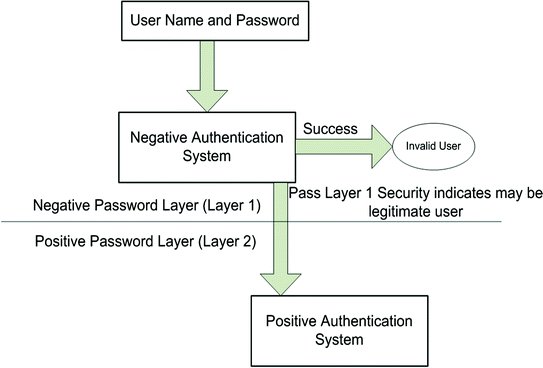
\includegraphics [width=15cm]{negative_password_architecture.png}
	\caption[Architektur zur Authentifizierung mit einem 'Negative Authentication System']{Architektur zur Authentifizierung mit einem 'Negative Authentication System'}
	\label{fig:negative_password_architecture}
\end{figure}

In der self-region sind die Passwortdaten beherrbergt. Diese Daten werden von der weitaus größeren non-self-region 'umschlossen', in der sich die Anti-Passwort-Detectoren befinden.
Während man \ac{nas} verwendet, ist es angebracht die Passwort-Profile und die Anti-Passwort-Profile auf zwei voneinander getrennten Servern zu bewahren. Dabei finden wie auf der Abbildung 2.2 zu sehen zwei Authentifizierungen statt. Bei der Ersten wird der Request mit der Datenmenge der Anti-Passwörter verglichen. Gibt es ein Match, ist der eingeggangene Request invalide. Auf diesem liegen die Detektoren für die Anti-Passwörter, die bei der Authentifizierung die Gülltigkeit der Anfrage erkennen, ähnlich wie die T-Helferzellen die Gülltigkeit von anderen Zellen im menschlichen Körper erkennen.

Dieser ''getrennte Server Ansatz`` für die Negativauthentikation besitzt gewisse Vorteile zu der Posoitivauthentifikation. Zunächst ein Mal ist es in der Lage bereits vor der eigentlichen Prüfung nach der Korrektheit des Passwortes invalide Requests abzufangen, die den zweiten Layer nie erreichen. Dies hat sich bereits als zielbringend erwiesen \cite{A14}. Außerdem sind die Daten des Nutzers hinter einem von außen nicht zu erreichenden Server versteckt, der nur mit dem ersten Layer kommuniziert. 'Guessing attacks' also Angriffe, die auf der Erratung von Passwörtern basieren, werden damit zu hoher Wahrscheinlichkeit verhindert \cite{A11}.

\textbf{Adaptive multi-factor-authentication (A-MFA)}

Da Nutzer durch mobile Technologien immer mehr Zugriff auf Online Services erhielten, entwickelte sich der Stand der Forschung immer mehr in Richtung verschiedener Authentifizierungsverfahren, unter denen der User eine Auswahl für sich treffen muss um seine Identität zu bestätigen \cite{A11}. Die Auswahl an Authentifizierungsfaktoren die dem Nutzer von Anwendungen präsentiert werden, entscheidet letzlich über die Performance von MFA's \cite{A11}. Daraus resultiert, dass die zufällige (oder Selbe) Auswahl von Verfahren für die MFA die Vertrauenswürdigkeit beeinträchtigen, da die Auswahl erratbar wird und bei entsprechenden Exploits auch unsicher. 

Die Auswahl der Verfahren findet zunächst aufgrund der Möglichkeiten eines Nutzers statt, demnach wird ermittelt welche Umgebung (welches Betriebssystem, welches Kommunikationsmedium und historische Daten) der Nutzer verwendet \cite{A15}. Um eine sichere Lösung für eine adaptive MFA zu entwickeln, muss die Erratbarkeit von dem Set an Authentifikationsmöglichkeiten verhindert werden. Dies bedeutet, dass es nicht möglich sein darf vordefinierte Muster für einen speziellen Nutzer mit einer speziellen Umgebung vorrauszusagen \cite{11}.

\section{Zielsetzung}
Passwörter können der allumfassenden sicheren Authentifikation nicht mehr gerecht werden. Es braucht weitere oder gänzlich andere Methoden, um die Identität eines Nutzers zu schützen. Die Menschheit benötigt einfache und unkomplizierte Methoden, die ihnen nicht das Gefühl geben allumfängliches technisches Know-How besitzen zu müssen, um die eigenen Daten im Internet zu schützen. Es sollte zum konsens werden, dass es bequeme Mechanismen für jeden Nutzer gibt. Je nach Gewichtung der Relevanz der Daten in den Kriterien Sicherheit, Bequemlichkeit und Datenschutz gibt es Möglichkeiten dies zu bewerkstelligen. Dies muss sowohl den Dienstbetreibern als auch dem Endnutzer bewusst werden. Nur die Erkenntnis über ein vorhandenes Problem kann zur Besserung führen und ist der erste Schritt. Nur so kann das Passwortproblem ein für alle Mal gelöst werden.

Ziel dieser Abschlussarbeit ist es eine Möglichkeit der Authentifikation zu spezifizieren, die im Jahre 2020 keine utopischen Szenarien beschreibt, die die Voraussetzungen für eine sichere, bequeme und datenarme Authentifikation erfüllt. Ziel ist es auch, den Leser in die Sicht des Angreifers auf Systeme einzuweisen, sodass im Idealfall automatische Schutzreaktionen wie das Wählen von sicheren Passwörtern hervorgerufen, wenn nicht sogar eine der beschriebenen FIDO2 Verfahren wie der erste oder sogar der zweite Faktor, verwendet werden. Der Prototyp soll die verschiedenen Authentifizierungsmöglichkeiten veranschaulischen und präsentieren, um dem Nutzer die Wahl auf eines der Verfahren zu erleichtern. Gleichzeitig ist eines der Hauptziele dieser Arbeit auch die Grenzen von 'modernen' Authentifizierungsverfahren aufzuzeigen und auf dessen Nachteile hinzuweisen. Inwiefern eine Kombination dieser vorhandenen Verfahren, Probleme löst und welche minderen Probleme dabei entstehen soll ausführlich erläutert werden. Jeder Nutzer besitzt persönliche Daten, an die kein Angreifer bzw. kein Dritter gelangen soll. Der Schutz dieser Daten sollte jedem Individuum selbst wichtig sein, um in den nächsten 5 bis 10 Jahren auf Besserung zu hoffen. Nicht nur technisch muss die Menscheit mit dem neuen digitalen Zeitalter umgehen und sich absichern können, sondern auch auf die menschliche Komponente muss von jedem selbst geachtet werden.

Dennoch sollte erwähnt sein, dass diese Arbeit nicht darauf abzielt jede mögliche vorhandene Authentifikationsstrategie zu durchleuchten. Erläutert werden die klassiche User-ID und Passwort Authentifikation und dem Gegenüber stehen die meistgenutzen Verfahren, die meist eher auf private Schlüssel, Besitz oder Biometrie setzen. Auch ist es ein Nicht-Ziel dieser Arbeit das Resultat auf eine einzige perfekte Lösung zu dezimieren und diese zum neuen Standard zu erklären. Viel mehr soll es dem Leser durch eine tabellarische Auflistung von Vor- und Nachteilen jeder Methodik selbst überlassen sein, welche Authentifikationsmethode ausgewählt wird.

% !TeX root = ../my-thesis.tex
\chapter{Grundlagen}

\section{Datenschutzkriterien}
\subsection{IT-Grundschutz}
Je nach Grundwert definiert der IT-Grundschutz welchen Schutzbedarf ein bestimmtes Asset oder ein Prozess besitzt. Allgemein kategorisiert werden die Schutzbedarfskategorien nach:
\begin{itemize} 
\item normal (Schadenauswirkungen begrenzt bis überschaubar)
\item hoch (Schadenauswirkungen könnten hoch bzw. beträchtlich sein)
\item sehr hoch (Schadensauswirkungen können ein existenziell bedrohliches Ausmaß annehmen
\end{itemize}
Bei dem Prototypen wird die allgemeine Schadensauswirkung wohl im Bereich normal liegen, da keine persönlichen Daten verarbeitet werden bzw. nur so viele Daten vom User benutzt werden, wie zwingend notwendig. (Nach dem Need-To-Know Prinzip) Sollte die Webseite oder Teile der Webseite publiziert bzw. im Business - Umfeld genutzt werden, muss eine Neubewertung der Daten nach Vertraulichkeit, Integrität und Verfügbarkeit stattfinden. Vor allem muss darauf geachtet sein, dass Daten über Fingerabdrücke verschlüsselt und Passwörter im gehashten Zustand in Datenbanken persistiert werden. Bei Kompromittierung des Hauptrechners, welches die größte Bedrohung in diesem Szenario darstellen würde, droht ein Data Breach mit dem Angreifer diese Daten weiterverwenden können. Durch Verschlüsselungen durch Schlüssel, die nicht auf dem Hauptsystem (oben u.a als Hauptrechner benannt) liegen. Gleichzeitig sollten die genutzten Verfahren insgesamt mathematisch sicher sein, auf veraltete Verschlüsselungsverfahren ist zu verzichten. Dies gillt auch für Hashes wie MD5, die mittlerweile durch sehr große vorgerechnete Tabellen erraten werden. \\\\
Im Falle einer Kompromittierung besäße der Schutzbedarf der Daten innerhalb der Datenbank, welche nicht gehasht oder anderweitig verschlüsselt sind, die Kategorie 'sehr hoch'. Eine Kompromittierung kann für das Unternehmen einen Imageschaden sowie weitreichende juristische Klagen zur Folge haben. Je nach dem wie kompliziert die Ursprungsdaten sind und welcher Hashingalgorithmus in Kombination mit Salt und Pepper genutzt wurde, können diese Daten an die Öffentlichkeit gelangen und Angreifer können die Passwörter für andere Dienste nutzen. Die Wahrscheinlichkeit für diesen Schaden ist noch vergleichbar niedrig, weshalb die Schadensauswirkung hoch statt sehr hoch ist. Beim Prototypen wird darauf geachtet werden, dass die Antwort zu möglichen Sicherheitsfragen auch verschlüsselt bzw. gehasht gespeichert werden und die Frage nicht in der Datenbank im Klartext steht sondern nur eine Zahl ist, die von der Webseite interpretiert wird und nie öffentlich gezeigt wird. \\
Der IT-Grundschutz definiert drei Arten der Absicherung. Die Basis-Absicherung ist relevant für Institutionen die einen Einstieg in den IT-Grundschutz suchen und relativ schnell alle relevanten Geschäftspozesse mit einfach umzusetzenden Basismaßnahmen sichern wollen. Die Kern-Absicherung konzentriert sich auf besonders wichtige Geschäftsprozesse und vertieft sich in die Sicherung dieser. Von einer Standard-Absicherung spricht man, wenn alle empfohlenen IT-Grundschutz-Vorgehensweisen durchgeführt werden. Sie beschreibt den allumfassenden Schutz der Prozesse und Bereiche der Institution. [9]

\subsection{ISO 27001}
Zunächst einmal muss unterschieden werden zwischen dem Standards ISO 27001 und der Zertifizierung von ISO 27001 auf Basis des IT - Grundschutzes. Im Grundansatz sind diese beiden Ansätze soweit kompatibel, da sie beide ein \ac{isms} beschreiben, um Risiken in der Informationssicherheit zu dezimieren (oder im besten Fall zu eliminieren). Gleichzeitig beschreiben beide eine Kontinuität in der regelmäßigen Überprüfung und Neubewertung dieser Risiken. Ein wesentlicher Unterschied zwischen den beiden Standards liegt in der Risikoanalyse. Während beim BSI-Grundschutz eine Risikoanalyse nur in besonderen Fällen erforderlich ist, ist sie beim Standard ISO 27001 ein fester Bestandteil, an das keine Bedingungen geknüpft sind. Wobei streng genommen häufig der eigentliche Schriftzug zur Risikoanalyse in der Norm ISO 27005 steht und darauf häufig verwiesen wird. Gleichzeitig sei laut Dr. Markus a Campo der Standard ISO 27001 mehr an dem Management der Informationssicherheit interessiert, wogegen der BSI-Grundschutz sich auf die detaillierte Vorgehensweise zur Minimierung von Risiken stütze. Unabhängig vom gewählten Standard sei es außerdem sinnvoll, die eigene Sicherheit in regelmäßigen Abständen zu überprüfen.
Laut dem \ac{bsi} ist die ISO 27001 Zertifizierung auf Basis des IT-Grundschutzes für sowohl Standard als auch die Kern-Absicherung möglich. [8] Die Zertifizierung auf Basis des IT-Grundschutzes erfüllt

\section{Authentifizierungsmethoden}
\subsection{Klassische Passwörter}
\subsection{Einmalkennwörter}
\subsection{Authentifizierung über Schlüssel}
\subsection{Biometrisierte Authentifizerung}

% !TeX root = ../my-thesis.tex
\chapter{Konzeption}
\section{Prototypenaufbau}
Das Ziel des Prototypes ist es, wie eingangs erwähnt, vorhandene Authentifizierungsverfahren abseits der klassischen UserID / Passwort Methode zu begutachten und dessen Schwächen aufzudecken. Der Prototyp beschreibt eine einfache Webseite, die aus dem globalen Internet erreichbar sein wird und zwei Eingabefelder und einen Loginbutton besitzt. Die unterschiedlichen Methoden der Authentifizierung wählt man über ein Dropdownmenü über dem Login - Button. Je nach Authentifizierungsverfahren werden kleine Popup-Boxen sichtbar, die die weiteren Schritte für die Authentifikation erläutern. So muss bei der zwei Faktor Authentifizierung anhand von einem Fingerabdruck weder ein Username noch ein Passwort eingegeben werden. Die Webseite muss lediglich auf die Schnittstellen des Betriebssystems zugreifen, um den Nutzer zu authentisieren. Wie der Nutzer eingangs den Fingerabdruck eingerichtet hat, spielt für die Webseite keine Rolle.
Ein Teil des Prototypen soll die gewählten Methoden demonstrieren. Neben einer erfolgreichen Demonstration der Authentifizierung sollen nach jeder Methode auch Kennwerte ausgegeben werden. Einer davon soll zum Beispiel die Zeit von der ersten Eingabe in ein Eingabefeld bis zur Authentifizierung in Sekunden zählen und anzeigen. Weitere Messwerte sind denkbar und werden sich bei der Implementation ergeben. \\
\\
Neben den vorhandenen Methoden soll die eigene Architektur aufgebaut werden, die sich an vorhandenen Authentifikationsmöglichkeiten bedient. Die UserID und das Passwortfeld sind beim ersten Aufruf der Seite zwar zu sehen, müssen allerdings nicht zwingend für jedes der Verfahren genutzt werden, so kann es zum Beispiel bei einer besitzbasierten Authentifikation bereits reichen, den Besitz (z.B einen USB - Stick, welcher einen privaten Schlüssel beherbergt) im Computer einstecken zu haben und auf den Loginbutton zu drücken. Bei der Architektur muss zwingend eine Datenbank und ein Backend zur Webseite implementiert werden um einerseits die eigeggangenen Daten zu bearbeiten und andererseits in die Datenbank zu persistieren. Das Dropdownmenü zeigt die Authentifikation über biologischen Merkmale (Touch ID oder Face ID) nur sofern das Gerät, auf welchem der Prototyp bedient wir, einen entsprechenden Sensor und die entsprechende Software zur Verarbeitung besitzt.

\section{Auswahl der Authentifizierungsverfahren}
Neben des altbekannten \ac{totp} Verfahrens, wird das Secure Element und die E-Mail Authentifikation betrachtet. Dabei bedienen sich diese Verfahren aller drei Möglichkeiten der Authentifikation, dem Wissen, dem Besitz und der körperlichen Merkmale. 

\section{Kriterien zur Bewertung des Prototypen}
\section{Architektur}

% !TeX root = ../Bachelorarbeit.tex
\chapter{Prototypischer Lösungsansatz}
\section{Implementationsdetails}
\begin{enumerate} 
\item \textbf{Client / Webseite}

Die Webseite besteht aus einer zur \ac{spa} ähnlichen Architektur, die ausschließlich Javascript und JQuery, also clientseitige Programmiersprachen nutzt. SPA's sind Webapplikationen, bei denen der Nutzer eine Seite betritt und diese nie wieder vollständig laden muss. Frameworks wie Angular, React oder VueJS basieren auf dieser Mechanik und nutzen Javascript und JQuery um die Ladezeiten einer Webseite durch Module zu reduzieren. Anstatt also die gesamte Webseite neuzuladen, laden diese Frameworks nur spezielle Bereiche der Webseite asynchron nach. In meinem Prototyp ist dies größtenteils der Fall, da neben der Hauptseite \textbf{index.html} eine weitere Seite existiert, auf die man bei erfolgreichem Login weitergeleitet wird: \textbf{secret\_panel.html}. Auch werden keine Module nachgeladen, sondern bei entsprechender Aktion nur Elemente innerhalb des DOM - Baums per id identifiziert und versteckt.

Beim Betreten von beiden Seiten der Anwendung findet eine Prüfung nach dem Session-Cookie (\textbf{user\_sid}) statt, die vom Server bei einer erfolgreichen Authentifikation im Header über 'Set-Cookie' als Response zurückkommt und vom Browser in folge dessen gesetzt wird. Der Aufruf der \textbf{index.html} Seite ist nicht möglich mit gesetztem Cookie und leitet den User auf \textbf{secret\_panel.html} weiter und umgekehrt genauso. Die Sicherung dieses Cookies auf Serverseite durch Prüfungen ist nicht Bestandteil dieser Arbeit, hier wird sich ledeglich auf den Loginprozess von Anwendungen konzentriert um dessen Schwächen und die Vorteile neuer Verfahren aufzuzeigen. Aktuell könnte ein Angreifer demnach selbst einen entsprechenden Cookie mit einem Wert setzen und das 'geheime Panel' erreichen. Bei weiter ausgereiften Webapplikationen wird bei jedem Request an den Server der Session Cookie mit einer temporären Map innerhalb des Backends abgeglichen. Befindet sich der Session Cookie nicht in dieser Map oder hat nicht genügend Rechte für diese Anfrage, erhält der Nutzer den Statuscode 401 (Unauthorized) zurück. So haben es etablierte Dienste wie 'Netflix' und 'Microsoft' bereits umgesetzt.

Aus der Forschungsfrage ergibt sich, dass die Webseite ausschießlich Javascript (oder auf Javascript basierende Programmiersprachen wie JQuery) zur Implementation der Programmlogik verwendet. Javascript selbst ist eine clientseitige Programmiersprache und gibt dem Nutzer den gesamten Code auf Webseiten preis. Demnach wurde bei der Anwendung darauf geachtet, alle clientseitigen Prüfungen, auch serverseitig zu implementieren. Zumindestens alle wichtigen Prüfungen, die sonst den Programmablauf verhindern würden oder sogar Serverabstürze zur Folge hätten. Nicht nur gibt Javascript den Code preis, über die Konsole (Unter Google Chrome und Firefox in den Entwickleroptionen des Browsers zu finden) lassen sich ganze Funktionen oder globale Variablen manipulieren. Variablen innerhalb von Funktionen können vom Angreifer nicht so leicht manipuliert werden.

Möglich ist es dennoch, den Inhalt dieser Funktion in eine andere Funktion zu schreiben, um die Variable dort auszutauschen. Um dem Nutzer nicht jede Funktion problemlos erreichbar zu machen, wurde bei der Implementation das Revealing-Module-Pattern angewendet, über die gewisse Variablen nicht im globalen Scope (window) sondern im Scope einer Funktion bleiben, die nur gewisse andere Funktionen in sich exportiert und als eine Art Schnittstelle fungiert. Auf dieses Pattern wird im Folgenden näher eingeggangen.

Das Design der Webanwendung ist kein wesentlicher Punkt dieser Arbeit und deshalb schlicht gehalten. So besteht der Prototyp aus einer einfachen Webseite, die aus dem globalen Internet erreichbar sein wird und die zwei Eingabefelder und einen Loginbutton besitzt. Um sich die Designarbeit oder das Suchen von Icons und passenden Buttondesigns zu sparen wurde auf bekannte Frameworks wie Bootstrap4 und Funktionalitäten wie Flexbox gesetzt, die eine automatisches Rescaling und Positioning von Webseitenelementen beinhalten. So war es nicht nötig ein Loginformular zu designen sondern vorhandene Strukturen von Bootstrap für Buttons aller Art zu nutzen. Die unterschiedlichen Methoden der Authentifizierung wählt man über ein Dropdownmenü über dem Login - Button. Je nach Authentifizierungsverfahren werden kleine Popup-Boxen sichtbar, die die weiteren Schritte für die Authentifikation erläutern. Die Methode kann sowohl über das Dropdownmenü als auch über einen Klick auf die Pfeile links und rechts neben dem Dropdownmenü gewählt werden, die als Pagination zwischen den verschiedenen behandelten Verfahren fungiert. Ist man am Ende der drei Methoden, springt man wieder zur ersten Methode und andersherum.

Bei der Web Authentication gibt es eine Besonderheit. Die Webseite auf die Schnittstellen des Betriebssystems zugreifen, um den Nutzer zu verifizieren. Dieser Teil kann von meinem Prototyp nicht beeinflusst werden und wird vom CTAP2 innerhalb des FIDO2 Standards definiert. Dadurch entstehen teilweise merkwürdige und aus UX (User Experience) - Sicht höchst fragwürdige Interaktionen. So fragt das Betriebssystem zunächst (bei entsprechender Möglichkeit) nach einem PIN um den Nutzer zu registrieren. Drückt man nun die Escape-Taste erscheint ein Dialog um einen Sicherheitsschlüssel (ein externes Gerät) einzurichten. Beim Login wiederrum ist dies durch eine Dropdownliste schöner gelöst worden, wo der User alle möglichen Loginmethoden auf einem Blick sieht und diese Wählen kann. Während er bei der Registration keine Chance hat dies zu tun und immer erst ein PIN - Feld angezeigt wird. Auf die einzelnen behandelten Verfahren wird in späteren Kapiteln noch genauer eingeggangen, da werden solche Schwierigkeiten aufgegriffen da dies nur eines von vielen 'Problemen' neuerer Verfahren ist: Die Abhängigkeit vom Betriebssystem.

\item \textbf{Server}

Der NodeJS - Server besteht aus einer REST Api, die keine Zustände speichert. Neben der Aufgabe des Cookie Managements und der Generierung von UUID's liefert er zudem die Schnittstelle zur Datenbank und verschiedene Funktionalitäten für die behandelten Verfahren Username \& Passwort, TOTP und Webauthn:

\begin{itemize}
 \item \textbf{/logout} - POST - Löscht den Session-Cookie (und damit die Session des Nutzers) und leitet ihn auf die Loginseite \textbf{index.html} weiter.

 \item \textbf{/get\_public\_key} - GET - Liest den öffentlichen Schlüssel des Servers ein und gibt diesen in einer JSON - Struktur zurück. Ist wichtig für die Username \& Passwort - Authentifizierung.

 \item \textbf{/password/login} - POST - Nimmt einen mit dem öffentlichen Schlüssel des Servers verschlüsselten Usernamen und Passwort entgegen und entschlüsselt diese mit dem privaten Schlüssel. Im Anschluss darauf wird in der Datenbank über einen gepoolte Query (eine Anzahl an Verbindungsprozessen zur Datenbank) nach dem Nutzer gesucht. Wurde dieser gefunden, erstellt der Server einen SHA512 - Hash aus dem Passwort (aus dem Request) und dem Salt des Users (aus der Datenbank) indem die \textbf{hashString} - Methode aufgerufen wird. Diese arbeitet mit der crypto Library um den Hash zu generieren und bezieht den Pepper des Servers mit ein. Sofern die Hashes aus der Datenbank und der soeben Generierte übereinstimmen, erhält der Nutzer die Response 200 und den Text ``OK''. Gleichzeitig wird wie bei jeder anderen Authentifizierungsmethode die \textbf{createSessionCookie} - Methode aufgerufen um den Session-Cookie (eine zufällige UUID) im Header zurück an den Nutzer zu senden, sodass dieser ihn im Browser.
 \newpage
 
 \item \textbf{/password/create\_password\_hash} - GET - Nimmt eine Zeichenkette des Nutzers entgegen und erstellt einen Password-Hash für den Nutzer, der manuell in die Datenbank persistiert werden kann. Ist als 'Quality of Service' Funktion zu verstehen, um es dem Administrator einfacher zu machen, Passwörter zu erstellen, die bei Vergleich einen gülltigen Hash ergeben.
 
 \item \textbf{/totp/check\_username} - POST - Diese Methode dient lediglich der Prüfung, ob der Nutzer die TOTP Authentifikation mittels zufälligem SECRET bereits gegenüber der Webseite validiert hat. Das Datenbankfeld 'totp\_activated' wird hier geprüft, ist der Wert 1 (stehen für das boolsche 'wahr') liefert der Server den Text ``Success'' zurück, das der Client deutet um nur das Feld für den sechsstelligen OTP Code anzuzeigen. Hat das Feld allerdings den Wert 0, wird entweder (sofern noch nicht vorhanden im Feld 'totp\_secret') ein neues Secret erstellt und in der Datenbank für diesen Nutzer persistiert. Gleichzeitig für eine URL beginnend mit otp:// erstellt, um diesen zusammen mit einem Base 64 enkodierten QR Code an den Client geschickt, der dies dem User präsentiert. Es wurde sich hier bewusst dazu entschieden, diese Schritte auf Serverseite vorzunehmen. Möglich wäre es auch auf Clientseite gewesen, wäre aber mit einem Mehraufwand verbunden, welches hier verhindert werden sollte.
 
 \item \textbf{/totp/check\_token} - POST - Nimmt den Usernamen des Nutzers und einen sechsstelligen TOTP Token entgegen. Sucht im Anschluss darauf in der Datenbank nach dem Nutzer und prüft über die Library 'otplib' ob der eingegebene TOTP - Token zum secret in der Datenbank valide ist. Dieser Schritt findet sowohl bei der Registration als auch beim Login statt. Wenn das Feld 'totp\_activated' also 0 ist, wird es bei der ersten Authentifikation auf 1 gesetzt und der Nutzer wird eingeloggt. (Session-Cookie wird gesetzt und nutzer weitergeleitet)
 \newpage

 \item \textbf{/webauthn/generate-attestation-options} - POST
 Liefert dem Nutzer die verschiedenen Registrieroptionen für die Web Authentication mittels WebauthnAPI. Dabei wurden verschiedene Optionen gesetzt, die im folgenden erklärt werden und die der User im Body der Response als JSON - Objekt erhält.
 
 \begin{lstlisting}[language=json,firstnumber=1]
        {
            rpName: PROJECT_NAME,
            rpId: WEBAPP_ORIGIN,
            userID: queryRes.rows[0].id,
            userName: username,
            userDisplayName: username,
            attestationType: 'none',
            authenticatorSelection: {
                requireResidentKey: false,
                userVerification: "discouraged",
            },
            excludedCredentialIDs: userAuthenticators.map(dev => dev.credentialID),
        }
\end{lstlisting}

\textbf{rpName:} rp steht hier bei für Relying Party. Das ist der Name, der später auch im Registrierungsdialog als 'Webseiteninhaber' gelistet wird.

\textbf{rpId:} Die Relying Party Id bekomtm eine URL, auf der Sich der Nutzer registrieren möchte. In unserem Falle ist dies 'localhost' ohne Zusätze wie das Protokoll oder der Port. Diese Variable ist vor allem für Webseiten im Netz wichtig, sodass ein Angreifer nicht per Pishing den Nutzer zur Registrierung auf einer anderen Webseite bringt. Die Registrierung schlägt clientseitig fehl, wenn die rpId und die Webseitenaddresse (Damit ist nicht die Domain sondern die wahrliche IP-Addresse gemeint) nicht übereinstimmen. Beim Wert 'localhost' sendet der Server diesen Teil der JSON - Abfrage nicht mit, da es localhost aus Testgründen nicht prüft. Gleichzeitig erzwingt Webauthn ausschließelich für diese rpId keine sichere Verbindung.

\textbf{userID:} Das ist die ID des Nutzers die verifiziert wird, meist eine fortlaufende Ganzzahl.

\textbf{userDisplayName:} Das ist der Name, der beim Registrieren als Username gelistet wird.

\textbf{attestationType:} Der Server definiert, wie viele Informationen über den Authenticator er im attestation statement haben möchte. Das attestation statement erhält er nach dem der User sich mit einem Authenticator registriert hat und ist ein wichtiger Bestandteil des Objekts welches den Server im Nachhinein über eine erfolgreiche Registration benachrichtigt. Ferner ist der öffentliche Schlüssel des Nutzers in diesem Objekt lokalisiert, den der Server dann in der Datenbank persistiert. 'none' bedeutet hierbei, dass keinerlei Informationen erwünscht sind. 'indirect' als Option würde dem Nutzer erlauben selbst zu entscheiden wie viele Informationen er preisgibt bzw. könnte er eine anonymisierte CA verwenden um sein Zertifikat auszustellen und 'direct' als Option würde die Daten direkt vom Authenticator ohne einen Eingriff des Nutzers erwarten.

\textbf{authenticatorSelection:} Das sind verschiedene Optionen um den verwendeten Authenticator zu bestimmen. Das Argument 'requireResidentKey' bestimmt hierbei darüber, ob ein Authenticator benutzt werden darf, der selbst nicht in der Lage wäre einen privaten Schlüssel auf dem Betriebssystem zu sichern und dem Server in folge dessen einen öffentlichen Schlüssel zu senden. Die 'userVerification' ist im Prototyp nicht erzwungen also 'required' sondern 'discouraged', es obliegt also dem Betriebssystem und dem zu authentifizierenden Gerät / und der initialen Konfiguration zu entscheiden, ob der Nutzer sich gegenüber seines Authenticators verifizieren muss. In dem Beispiel eines bereits sicheren FIDO2 - USB Sticks könnte dies zum Beispiel nicht vom Nutzer gewünscht sein.

\textbf{excludedCredentialIDs:} Dies ist eine Liste von credentialID's die in der Datenbank im Feld 'webauthn\_authenticator\_data' als JSON - Sturktur persistiert sind. Sie dient dazu, bereits registrierte Methoden nicht erneut anzuzeigen, funktioniert dennoch nicht zuverlässig.
\end{itemize}

\item \textbf{Datenbank} (Schadensauswirkungen können ein existenziell bedrohliches Ausmaß annehmen
\end{enumerate}

\section{Erfolgreiche Authentifikation}




% !TeX root = ../Bachelorarbeit.tex
\chapter{Auswertung}
Das Passwort war jahrzehntelanger Vorherrscher in der Authentifikation im Web und schien eine kurze Weile auch sicher. Nach dem die ersten Bruteforce-Angriffe auf Formulare angeggangen wurden, mussten neue Regeln für Passwörter her. Der Nutzer durfte sie nicht mehr nach eigenem Ermessen wählen, da der Imageschaden durch z.B: die Infiltrierung einer wichtigen hochrangigen Person eines Unternehmens zu groß wurde. Die Fälle der Data-Breaches und Leaks wurden trotz Passwort-Policy Ansätzen und der Einführung des zweiten Faktors nicht weniger sondern im Gegenteil: Sie häuften sich mehr und mehr. Passwörter wurden theoretisch durch erzwungene Sonderzeichen und einer Mindestlänge komplexer, allerdings wurde genau hier nicht mit der Natur des Menschen gerechnet. Da Formulare nun mehr und mehr Passwörter abzulehnen schienen, beggangen Menschen die Sicherheitsfeatures instinktiv zu umgehen. Darauf folgten die 'zeitlich begrenzten Passwörter', welche aus dem selben Grund, dem Bequemlichkeitsproblem, scheiterten. Neuere Verfahren sollten die alteingesessenen ersetzen oder zunächst ein Mal unterstützen. Die neue Zeit des Smartphones ermöglichte den Nutzern ihre Geräte zur Authentifikation zu nutzen, wofür sie davor kostspielige Geräte kaufen hätten müssen. Die Zeit der Einmalkennwörter brach an und Apps wie der Google Authenticator oder der Microsoft Authenticator gewannen mehr und mehr an Popularität. Mit der Zeit wurden allerdings auch diese 'weiteren Schritte' zur Authentifikation dem Nutzer zu lästig. Vor allem wichtige Dienste wie Banken führen kein Sessionmanagement und nötigen den User häufig zur mehrmaligen Authentifikation während einer Sitzung. Und genau an diesem Standpunkt setzen die neuesten Verfahren an. Die Webauthentikation ist dem Passwort in vielen Dingen überlegen. Zunächst ein Mal werden nur noch zufällig generierte Schlüssel ausgetauscht. Außerdem geschieht das über Challenge-Response-Verfahren wodurch Wiederholungsangriffe vermieden werden. Der Nutzer ist nicht mehr der Kern der Authentifikation sondern der Authentifikator (das Gerät) selbst. Bei neueren public-private-key Verfahren gibt es keine Geheimnisse, die auf einfachste Art und Weise (z.B: über Keylogger, Trojaner oder Shoulder Surfing) entwendet werden könnten. Die Verantworung zur sicheren Aufbewahrung von Passwörtern hat sich vom Nutzer auf die Betriebssysteme verschoben, die die privaten Schlüssel sichern müssen. Die \ac{mitm} - Problematik schien immernoch nicht gelöst. So ist die Kommunikation dann durch den \ac{mitm} angreifbar, wenn der Aussteller des Zertifikats nicht bekannt ist. Die Webauthentikation bietet einem Mann in der Mitte allerdings keine einfache Möglichkeit, die Identität des Nutzers anzunehmen.
\newpage

Abseits der Problematik bietet der FIDO2 - Standard mit Webauthn und CTAP2 die Kommunikation über verschiedenste Authentifikatoren und bietet damit potenziell sehr vielfältige Lösungsansätze für Authentifikationen im Webbereich.
Dennoch ist die Umsetzung des Hauptbetriebssystems Windows aus UX-Sicht nur suboptimal. Gleichzeitig ist die Implementation von Webauthn auf Clientseite zwar größtenteils schon möglich, auf Serverseite fehlt es bei Javascript basierenden Webseiten aber an ausgereiften Web-API's. Die Abstraktion der Vorgänge im Webauthn - Protokoll durch vorhandene API's (wie die genutze im Prototyp) hat den Vorteil, dass der Implementationsaufwand durch eine Senkung der Komplexität sinkt. Gleichzeitig muss bei Fehlern in der abstrahierten Bibliothek ein Mehraufwand an Verständnis dessen, was die Bibliothek macht, aufgetrieben werden. Gemessen daran, dass man das Protokoll allerdings nur einmalig implementieren muss und die FIDO-Alliance große Unterstützung für Webseiten für alle möglichen Programmiersprachen bietet, scheint dieses Argument entkräftigt.

Der Prototyp beweist zweierlei Dinge. Zunächst ein Mal ist es möglich, einen Nutzer bereits mit einem einzigen sicheren Faktor und dessen Nutzernamen zu authentifizieren. Das Passwort sollte im Jahre 2020 eher zur Ausnahme in der Sicherung und wenn überhaupt nur mit einem zweiten Faktor verwendet werden dürfen, sofern es dem User nicht möglich ist die sichereren Verfahren zur Authentifikation zu nutzen. Dies könnte zum Beispiel dann der Fall sein, wenn es dem Nutzer an den benötigten Geräten (der Hardware) fehlt oder die Hardware nicht mit dem Betriebssystem kompatibel ist. Außerdem beweist die Webseite, dass die Implementation der neueren Verfahren keine große Hürde darstellt und einem potenziellen Unternehmen auf lange Sicht viele Supportanfragen zwecks vergessenen Passwörtern oder gekaperten Accounts ersparen kann.

Es gillt noch zu schauen, inwiefern die Anforderungen aus dem Kapitel für sichere Webseiten vom Prototypen erfüllt werden konnten:

\begin{itemize}
\item \textbf{Immer mehr Nutzer sorgen für mehr Authentifikationen pro Sekunde und damit für eine höhere Auslastung}

Bei der Wahl der Umgebung des Backends wurde bewusst NodeJS gewählt, das im Kern bereits eine asynchrone Verarbeitung hat. Das heißt das diese Programmiersprache und die genutzte Library 'ExpressJS' in der Lage sind, viele Anfragen verschiedenster Nutzer parallel zu bearbeiten. Die Anfragen blockieren sich nicht untereinander. Dazu besitzt der Prototyp bewusst keine statische Verbindung zur Datenbank sondern ein Pooling. Es baut also bei Serverstart einige (nicht spezifiziert) Verbindungen zur Datenbank auf. Sollte es mal sein, dass eine dieser Verbindungen abbricht, dann stürzt der NodeJS Server nicht ab sondern kann bei der nächsten Anfrage einfach eine neue Verbindung aus dem Pool für die Anfrage verwenden. Die Authentifikation von vielen verschiedenen Nutzern ist dem Prototypen dadurch problemlos möglich.

\item \textbf{Webseiten sind über das offene Netz zugänglich und bieten damit eine große Angriifsfläche für Brute-Force Angriffe}

Der Prototyp besitzt keine konkreten Vorsichtsmaßnahmen gegen Bruteforce - Angriffe. Dies müsste in Folgeversionen implementiert werden, da sonst eben genau die geschilderte Gefahr der Erratung von User Credentials über das Durchprobieren von Passwörtern groß ist. Bei dem Verfahren der Webauthn ist kein Schutz gegen Bruteforce - Angriffe nötig, da diese keine 'offenen Credentials' wie dem Passwort besitzen das erraten werden könnte. Anders sieht es bei der TOTP-Authentifikation aus, hier ist eine Brute-Force Gefahr sehr hoch, da der TOTP Code nur aus einer sechsstelligen Zahl besteht. Das sind genau 1.000.000 Möglichkeiten, die der Angreifer innerhalb von 30 Sekunden (alle 30 Sekunden zyklisch) ausprobieren muss. So würde er die Authentifikation durch ein Gerät umgehen können, dies muss in Folgeversionen verhindert werden und wurde zeitbedingt nicht implementiert. Auch war es geplant diesen Schutz anhand einer Firewall vor der Webseite zu stützen, wodurch dies programmatisch vernachlässigt werden könnte.

\item \textbf{Webseiten besitzen mehr Möglichkeiten als je zuvor um Nutzer zu authentifizieren, von dem muss sie aber erst Gebrauch machen}

Die Verfahren des 21. Jahrhunderts werden dem Nutzer wunderbar präsentiert und können von ihm für die Authentifikation genutzt werden. Bei der Username \& Passwortauthentifikation fehlt es an einer Registrierung. Abseits dessen, sind die TOTP und Webauthn Registration bereits sicher und bequem implementiert. Auch werden alle drei Kateogorien durch ihre entsprechenden Verfahren bedient.

\item \textbf{Webanwendungen speichern üblicherweise Nutzerkonten bzw. personenbezogene Daten}

Personenbezogene Daten werden vom Prototypen nicht gespeichert, da es sich hierbei nur um ein Modul einer Webanwendung handelt, ist dies allerdings auch nicht nötig. Andere Daten wie Passwörter werden mit einem sicheren Hashingverfahren (Salted and Peppered SHA256) in der Datenbank persistiert und sogar auf Clientseite wie empfohlen zusätzlich verschlüsselt und dann übertragen. Wie bereits erwähnt ist die Speicherung von Biometriedaten nicht nötig, da Webauthn nur einen zufällig generierten Hash als 'credentialID' persistieren muss um die Folgeauthentifikation des Nutzers zu erkennen.

\item \textbf{Webnutzer sind oft unvorsichtig mit Passwörtern und wählen zu leichte}

Dieser Punkt war recht schwierig zu verhindern, obwohl die Verfahren wie man ihn umsetzen kann bereits gut erforscht sind. Die Hauptproblematik von Passwörtern und Passwort Policies wird an diesem Punkt sehr klar. Egal welche Policy für Passwörter gewählt wird, dem Nutzer ist es möglich dennoch unsichere Passwörter zu wählen. Wählt man zu viele Richtlinien wird der Nutzer sich aufgrund seiner Beqeuemlichkeit auf kurz oder lang bewusst für diese Unsicherheit entscheiden. Nutzt man gar keine Policy dann ist dem Nutzer gar keine Grenzen an einfachen Passwören wie ``1234'' gesetzt. Der Prototyp hat nur eine simple Policy: Passwörter und Nutzernamen müssen eine Mindeslänge von 8 Zeichen besitzen. Dieses Problem kann nicht so richtig bearbeitet werden, da ein Nutzer im Zweifelsfalle immer seine Bequemlichkeit vor seine Sicherheit stellt was dann zu Identitätsdiebstahl usw. führt.
\end{itemize}

Zum Abschluss der Bachelorarbeit muss noch geklärt werden, welches Verfahren für welchen Nutzertypus geeignet ist. Auch wenn man dies nicht pauschalisieren kann, sollte man zunächst ein Mal klären welcher Nutzer welche Anforderungen stellt. Alle Internetnutzer, ob es nun ein erfahrener Entwickler, ein Casual Erwachsener oder Jugendlicher ist, haben Interesse an dem Schutz ihrer Daten. Auch wenn ihnen die Wichtigkeit ihrer Daten und die Gefährdung größenteils nicht bewusst sind. Jugendliche haben heutzutage nur in seltenen Fällen kein Smartphone und können somit das TOTP-Verfahren oder die Webauthn (falls von der Internetseite umgesetzt und untersützt) verwenden. Älteren Personen fehlt es womöglich an technischer Hardware, doch hier kommt die Authentifikation über PIN (sogenanntes self-signed-device) oder die Stimme am Rechner ins Spiel. Auch wenn kein externes Gerät wie ein Smartphone vorhanden ist, kann häufig bereits der eigene Rechner einige Authentifikationsmethoden unterstützen. Sollte man, aus gegebenen und teilweise genannten Gründen, keine Möglichkeit auf Alternativen zum Passwort besitzen, sollte das Passwort nicht als alleiniger Authentifikator verwendet werden dürfen. Ein zweiter Faktor ist aber nur strikt für das Passwort erforderlich, denn die anderen Verfahren sind nicht so großen Gefahren ausgesetzt wie es das Passwort ist. Die Öffentlichkeit muss sich der Wichtigkeit ihrer Identität bewusst werden, um die Entscheidung über Passwörter und dem erzwungenen zweiten Faktor nachzuvollziehen. Zuletzt bleibt noch zu erwähnen: Der Codename des Prototypen 'clsec' ist ein Kürzel der Wortschöpfung 'Clientless Login' und bedeutet so viel wie ``Die Authentifikation ohne Passwort'' und mach den Prototypen damit zum Beweis dafür, dass diese auch Zukunft hat.

% !TeX root = ../Bachelorarbeit.tex
\chapter{Ausblick und Fazit}
Die Userverifikation ist eine der größten Herausforderungen an Webanwendungen der Neuzeit und wird es voraussichtlich auch bleiben. Das Verfahren der Negativauthentifikation zeigt in welche Richtung zukünftige Verfahren wohl gehen: Man versucht die alteingesessenen Passwörter durch neue Denkansätze und Verfahren besser zu schützen. In diesem konkreten Beispiel macht man wortwörtlich das Gegenteil einer gewöhnlichen Authentifikation und versucht dadurch falsche Anfragen zu erkennen bevor der Server sie überhaupt prüfen muss. Zusätzlich scheint der Zufall in den Fokus zu kehren, während die gewöhnliche Multi-Fator-Authentifikation feste Auswahlmöglichkeiten bot, ist die A-MFA darauf spezialisiert dem User seinen Parametern zugeschnittene Möglichkeiten zu bieten. Das macht es Angreifern ungemein schwer, einen bestimmten Nutzer konkret anzugreifen - Da jeder Nutzer ein potenziell anderes Preset bzw. 'Profil' besitzen wird, das seine Authentifizierungsmöglichkeiten ergibt. Neben neuen Ansätzen muss sich die zukünftige Forschung wohl vermehrt mit der Haltung der Nutzer zum Thema Bequemlichkeit widmen. Neuere Verfahren, die aus technischer Sicht sehr sicher sind, können nicht bestehen wenn sie vom Nutzer nicht als angenehm bzw. bequem empfunden werden. Die Digitalisierung zwingt Webseitenbetreiber (durch öffentlichen Druck und Konkurrenz) dazu, alle vorhandenen Möglichkeiten zur Authentifikation anzubieten und dem Nutzer die Wahl dessen zu lassen. Das Selbe macht der Prototyp, der eine zufällige Webseite als Authentifikationsmodul absichern kann. Um die Verfahren (MFA) noch mehr abzusichern, wäre es in Zukunft nötig die Adaptivität zu steigern, indem die Verfahren dem Nutzer nur präsentiert werden, falls das Userprofil und das vorhandene Betriebssystem / Gerät dies hergibt. Die Authentifikation gelingt den Menschen der Zukunft recht gut, sie muss dem Nutzer nur noch bequem gemacht und angeboten werden. So kann das Passwortproblem mit neuen Verfahren gelöst werden.


\cleardoublepage

\printbibliography % Print the bibliography
\cleardoublepage

\appendix % Begin the appendix. Chapters begin with letters
% \pagenumbering{Roman} %page numbers as capital roman numbers
\setcounter{page}{1} % restart page numbers from one
% !TeX root = ../my-thesis.tex
\chapter{\appendixname}\label{sec:appendix}
\section{Ergänzende Informationen}
\blindtext[3] % include the appendix
\end{document}
% ----------------------------------------------------
